% !Mode:: "TeX:UTF-8"
%!TEX program  = xelatex

%\documentclass{cumcmthesis}
\documentclass[withoutpreface,bwprint]{cumcmthesis} %去掉封面与编号页
\usepackage{CJK}
\usepackage{fancyhdr}
\usepackage{url}

\title{基于改进的智能遗传算法的RGV动态调度策略}
\tihao{B}
\baominghao{201818004121}
\schoolname{中南大学}
\membera{张震东}
\memberb{朱正}
\memberc{杜婷}
\supervisor{贺福利老师}
\yearinput{2018}
\monthinput{08}
\dayinput{22}

\begin{document}

 \maketitle
 \begin{abstract}
CNC物料加工过程中不发生故障时,为使加工产品数目最多,我们首先从排队论的思想:先到先服务、以及服务时长最短两个角度考虑使RGV每一步的动作都尽可能节省时间,得到较优解;接着,由于局部最优不一定是全局最优,但是考虑到采用枚举法进行全局搜索的效率问题,我们以求得的较优解为初始化种群,加工产品数目为适应性函数,根据实际情况增加良性变异以及优越种群发生繁殖的可能,设计基于改进遗传算法的随机全局最优搜索算法。特别的,在两道工序的情况下,需要考虑RGV当前状态对下一状态的影响。

加工需要两道工序且考虑故障的情况与两道工序不考虑故障的情况的模型类似,但不同的是,每次RGV为CNC上下料时,该CNC在接下来的工作时间内有一定可能性发生故障。和一道工序有故障的情况相同,依然生成随机数来判断是否会发生故障,以及发生故障的时刻和时间长度。
















\keywords{RGV\quad  CNC\quad   改进的遗传算法\quad  随机数}
\end{abstract}

%目录
\tableofcontents
\newpage



\section{符号说明}
\begin{center}
\begin{tabular}{cc}
 \hline
 \makebox[0.3\textwidth][c]{符号}	&  \makebox[0.4\textwidth][c]{意义} \\ \hline
 $n_{1}$	    & 一道工序加工的总产品(个) \\ \hline
 $n_{2}$	    & 一道工序加工的总产品(个) \\ \hline
 $n_{1(i)}$	    & 一道工序情况下,第i台CNC加工的产品(个) \\ \hline 
 $S_i^j(S_i=1,...,8)$	    & 第j代的第i次操作后的对象CNC  \\ \hline
 $O_{c(i)},O_{t(i)}$	    & RGV对第i台CNC下料(O)操作次数(c)/时间(t)  \\ \hline
 $I_{c(i)},I_{t(i)}$	    & RGV对第i台CNC上料(I)操作次数(c)/时间(t)  \\ \hline
 $M_{c(i)},M_{t(i)}$	    & RGV对第i台CNC移动(M)操作次数(c)/时间(t)  \\ \hline
  $C_{c(i)},C_{t(i)}$	    & RGV对第i台CNC清洗(C)操作次数(c)/时间(t)  \\ \hline

\end{tabular}
\end{center}

\section{问题分析}
\subsection{RGV运动规律}
\label{RGV运动规则}
\textbf{RGV的状态简化}

根据题意,在不考虑故障的前提下,为研究一道工序的物料RGV加工作业情况,首先由RGV的作业流程,我们发现RGV在工作中会出现5个状态:
\begin{enumerate}
\item 向发出信号的CNC移动
\item 等待CNC的工作信号
\item 为CNC上料
\item 为CNC下料
\item 清洗成料
\end{enumerate}

值得注意的是,除了RGV给任一CNC第一次上料外,在一道工序的物料加工作业情况下,为CNC下料、为CNC上料和清洗成料的过程一定是依次连续进行的,故以下将为CNC下料、为CNC上料和清洗成料状态合并成一个状态看待。因此,在道工序的无故障发生情况下,除了RGV给CNC第一次上料外,我们可以将RGV的五种可能状态转化为一下三种工作状态:
\begin{enumerate}
\item 向发出信号的CNC移动
\item 等待CNC的工作信号
\item 为CNC下料、上料、清洗成料
\end{enumerate}

\textbf{RGV的运动基本规律}

因为RGV在接收到CNC的上下料需求信号之后才会移动,所以移动的后续状态必为CNC上下料。又因为而某一次状态结束后所在的位置,的对象CNC
共有以下几个规律:
\begin{enumerate}
\item RGV移动的后续状态必为给CNC下料、上料、清洗成料
\end{enumerate}

\subsection{RGV调度策略数组模拟模型}

为了模拟RGV全程操作过程,方便编程和模型处理,根据RGV状态与规律分析,我们建立如下数组,以记录RGV的8小时全程操作过程。

\textbf{RGV调度策略的数组模拟模型定义与性质}

首先我们给出RGV调度策略的数组模拟模型的定义:
\begin{definition}[RGV调度策略的数组] 
定义如下数组$S$记录RGV调度策略 ,其中包含若干个元素$S_i$,其中$i$表示RGV的操作次数,$S_i$表示第$i$个元素操作的CNC代码,其中$S_i$的定义域为$[ 1,8 ]$,且$S_i$为正整数。
\begin{equation}
S=\{S_1,S_2,...,S_i,...\}(1\leq S_i\leq 8,S_i\in Z^*)
\end{equation}
\end{definition}
根据定义,我们运用RGV调度策略数组表示全程8小时的RGV移动策略。我们可以根据数组相邻元素的特点,得出RGV在这一个位置所进行的操作。
\begin{lemma} 
数组中任意两个相邻数之间仅有相等和不等两种情况。
\label{引理1}
\end{lemma}
\begin{lemma} 
RGV的相邻两个操作仅有等待和不等待两种情况。
\label{引理2}
\end{lemma}
根据引理,我们可以得出以下关于RGV调度策略数组的定理。
\begin{theorem}[重复等待定理] 
对RGV调度策略数组,要使$S_i=S_{i+1}$ ,当且仅当RGV在第$S_i$台CNC所对应的RGV传送带的位置等待指令。
\end{theorem}
\begin{theorem}[非重复移动定理] 
对RGV调度策略数组,要使$S_i\neq S_{i+1}$ ,当且仅当RGV在第$S_i$台CNC所对应的RGV传送带的位置非等待指令。也即,RGV在$S_i$台CNC所对应的RGV传送带的位置对$S_i$进行操作后,RGV没有在原地执行等待操作,而是直接执行移动操作前往$S_{i+1}$,对$S_{i+1}$执行相应操作。
\label{非重复移动定理}
\end{theorem}


根据\ref{RGV运动规则}得出的RGV的运动基本规律,可知定理\ref{非重复移动定理}中,$S_{i+1}$执行的操作必为给CNC下料、上料、清洗成料。

\textbf{RGV调度策略数组所对应的实际操作过程}

综上所述,相邻两个第 $S_{i+1}$至$S_i$台CNC所对应操作,有如下三种可能:
\begin{enumerate}
\item 若$S_i=S_{i+1}$ ,则表示RGV在第 $S_{i+1}$也即$S_i$台CNC等待;
\item 若 $S_i\neq S_{i+1}$,且$[\frac{S_i}{2}]\neq[\frac{S_{i+1}}{2}]$,则表示RGV先为第 $S_i$台CNC进行上下料和清洗后,需进行移动到达第$S_{i+1}$ 台CNC,再为第 $S_{i+1}$台CNC进行CNC下料、CNC上料和清洗成料操作(RGV可能要移动1,2,3个单位);
\item 若 $S_i\neq S_{i+1}$,且$[\frac{S_i}{2}]=[\frac{S_{i+1}}{2}]$,则意味着第  $S_i$台CNC和第$S_{i+1}$ 台在同一位置的轨道两侧,表示RGV先为第 $S_i$台CNC进行上下料和清洗后,无需移动,再直接为第 $S_{i+1}$台CNC进行CNC下料、CNC上料和清洗成料操作(RGV移动0个单位)。
\end{enumerate}

例如:S=(1,2,3,4,5,6,7,8,8)中,(1,2)表示关系2 ;(2,3)表示关系3 ;(8,8)表示关系1.


\begin{table}[!htbp]
\caption{数字及数字特征与其意义对照表}\label{数字及数字特征与其意义对照表} \centering
\begin{tabular}{cc}
\toprule[1.5pt]
数字及数字特征 & 意义 \\
\midrule[1pt]
 $S_i(S_i=1,...,8)$	    & 第i次操作后的对象CNC  \\ 
 $S_i=S_{i+1}$	    & RGV在第 $S_{i+1}$也即$S_i$台CNC等待  \\ 
 $S_i\neq S_{i+1}$且$[\frac{S_i}{2}]\neq[\frac{S_{i+1}}{2}]$	    & RGV对第 $S_{i+1}$台CNC进行下料、上料和清洗成料操作  \\ 
 $S_i\neq S_{i+1}$且$[\frac{S_i}{2}]=[\frac{S_{i+1}}{2}]$	    & RGV对第 $S_{i+1}$台CNC进行下料、上料和清洗成料操作  \\ 
\bottomrule[1.5pt]
\end{tabular}
\end{table}

综上所述,根据RGV调度策略数组与RGV运行轨迹的一一对应关系,我们得到的RGV调度策略数组可以完整的反应RGV运行轨迹。只需对RGV调度策略数组按照表\ref{数字及数字特征与其意义对照表}进行编译,即可得到RGV的完整运动信息,又因为CNC除了自身出现故障外,CNC的运行状态完全取决于RGV的运动信息。因此我们运用RGV调度策略数组,可以推算出RGV以及CNC的全部信息。

\subsection{四种情况分析}
\subsubsection{一道工序的无故障发生情况分析}


由RGV调度策略数组模拟模型,我们可以由RGV调度策略数组得到实际操作过程,也可以由实际操作过程得到RGV调度策略数组。根据题目要求,我们的优化目标为生产最多的产品的数学目标如\eqref{一道工序生产最多的产品}所示
\begin{equation}
Max\quad n_{1}=\sum_{i=1}^8 n_{1(i)}
\label{一道工序生产最多的产品}
\end{equation}

由于在一道工序的无故障发生情况下,每个CNC生产一个产品意味着进行一次下料操作和清洗操作。因此第i台CNC生产的产品数$n_{1(i)}$,可以用RGV对第i台CNC进行的下料操作次数$O_{c(i)}$或清洗操作次数$I_{c(i)}$体现,即:
\begin{equation}
n_{1(i)}=O_{c(i)}=C_{c(i)}
\end{equation}
所以有

\begin{eqnarray}
 & Max\quad n_{1}=\sum_{i=1}^8 O_{c(i)}\\
or, & Max\quad n_{1}=\sum_{i=1}^8 C_{c(i)}
\end{eqnarray}

\textbf{求解优值算法}

为了实现这一目标,我们可以基于排队论的思想,得到了两种得出较优解的算法,为得到全局最优解,而后可采用枚举算法和随机算法
\begin{itemize}
\vspace{6pt}
\item 算法一:先到先服务算法


\vspace{6pt}
\item 算法二:服务时长最短算法


\vspace{6pt}
\item 算法三:全局枚举算法

全局枚举法可以得出所有的可行解,但是运算量极大。在本题情况下,所有可行解的数量级大于$10^{100}$,由于运算量过大,我们放弃了这种算法。
\vspace{6pt}
\item 算法四:基于改进遗传算法的随机全局最优搜索算法

由于算法一和算法二得到的结果,是局部最优解,但不一定是全局最优解,因此我们应找出一种方法能找出目标的最优解。但全局枚举算法运算量巨大,故舍弃,我们需要一种运算量方法来寻找最优客。而遗传算法作为一种随机算法\upcite{bib:two},可以在较小的运算量下,得出相对较优的解。但对于本题,传统的遗传算法的编码方式和繁殖、变异方式不适用于本题。于是,我们需要对传统的遗传算法的编码方式和繁殖、变异方式依题意进行改良。


\end{itemize}















\subsubsection{一道工序的有故障发生情况分析}
针对CNC物料加工作业过程中可能发生故障的情况,我们根据问题中对于发生故障的大小和故障时间长度的假设,用计算机生成随机数,根据随机数的大小判定在某一次作业中是否发生故障,同时生成两个随机数决定故障发生时刻和故障时间长度,并与不考虑故障的CNC物料加工作业的模型结合,得到相应情况下CNC调度安排。






\subsubsection{两道工序的无故障发生情况分析}
在每台CNC加工的工序确定时,我们仍旧可以利用先到先服务算法和服务时长最短算法寻求较优的RGV动态调度方案,并计算这种方案下加工的产品数目。

与一道工序的无故障发生情况不同的是,在每个物料要进行两道工序的情况下,当RGV为进行第一道工序的CNC进行上下料作业后,它的下一个任务安排只能是等待CNC的指令或者为进行第二道工序的CNC上下料和清洗物料,但是,若RGV只为进行第一道工序的CNC进行上料作业后,它的下一个任务安排只能是等待CNC的指令或者为进行第一道工序的CNC上下料。基于此,我们对一道工序的无故障发生情况下的算法进行修正。

由于加工不同工序的CNC的数量以及位置的不同均会导致生产产品数目的不同。为了在8个小时内加工最多的产品数目,我们可以以每台CNC加工的工序为决策变量建立目标规划模型,寻求较优的CNC工序安排方案








\subsubsection{两道工序的有故障发生情况分析}












\section{模型的求解}
\subsection{一道工序的无故障发生模型}

为了求得一道工序的无CNC故障发生的最优智能RGV动态调度策略,根据问题分析中的\eqref{一道工序生产最多的产品}式,


\subsubsection{先到先服务算法} 
为了方便叙述算法,我们使用以下变量

(1)8台CNC分别已经加工当前物料的时间  $A = \left[ {A(1),A(2),...,A(8)} \right]$

(2)RGV累计运行时间  $T$,其初始值为0,且要满足运行时间小于8小时

(3)CNC加工完成一个一道工序的物料所需时间  ${T_0}$

(4)物件上下料时间  $t\_add$,清洗时间  $t\_wash$,RGV移动时间  $t\_move$
首先为了判断RGV的下一个状态,需要判断是否有发出需求信号的CNC以及发出需求信号的CNC数量。
根据RGV的作业流程,我们得到如下结论
\begin{itemize}
	\item 如果  $Ai < {T_0}$,则表示没有CNC发出需求信号,RGV原地等待。等待时间为  $\tau  = \min \{ {T_0} - A(i)\} $, 的增加量  $\Delta T = \tau $
	\item 如果  $Ai \ge {T_0}$,则表示有CNC发出需求信号,RGV需要为该CNC上下料。上下料后  $Ai = 0$
\end{itemize}

根据“先到先服务”的模式的要求,在RGV位于第 台CNC旁准备移动时,找出之前最早发出需求信号的CNC,由于越先发出信号的第 台CNC对应的  $Ai$越大,所以找出最先发出信号的CNC的方法为:

设第  $j$台CNC满足要求,则  $A(j) = \mathop {\max }\limits_{A(k) > {T_0}} A(k)$。  $T$的增加量  $\Delta T$为对应的移动时间,上下料和清洗时间之和。其中移动时间又可以由题中与移动距离的关系得到,移动距离为  $(\left| {\left\lceil {\frac{{S(i)}}{2}} \right\rceil  - \left\lceil {\frac{j}{2}} \right\rceil } \right| + 1)$,上下料后  $Aj = 0$
只要累计运行时间 满足小于8小时,就一直往复进行寻找。



\subsubsection{服务时长最短算法}

对于第j台CNC,当  \[Aj \ge {T_0}\]时该CNC即进入等待状态,等待时间为RGV到达时的  \[Aj - {T_0}\],而  \[Aj\]为RGV移动时间,清洗时间,上下料时间,加工时间之和,又加工时间相同,所以寻找等待时间最短的CNC方法是:  \[Aj = \mathop {\min }\limits_{Ak > {T_0}} \{ {\rm{ }}time\_add + time\_move + time\_wash\} \],其中移动时间又可以由题中与移动距离的关系得到,移动距离为  \[(\left| {\left\lceil {\frac{{S(i)}}{2}} \right\rceil  - \left\lceil {\frac{j}{2}} \right\rceil } \right| + 1)\],上下料后  \[Aj = 0\]



\subsubsection{基于改进遗传算法的随机全局最优搜索算法}

\begin{figure}[!h]
\centering
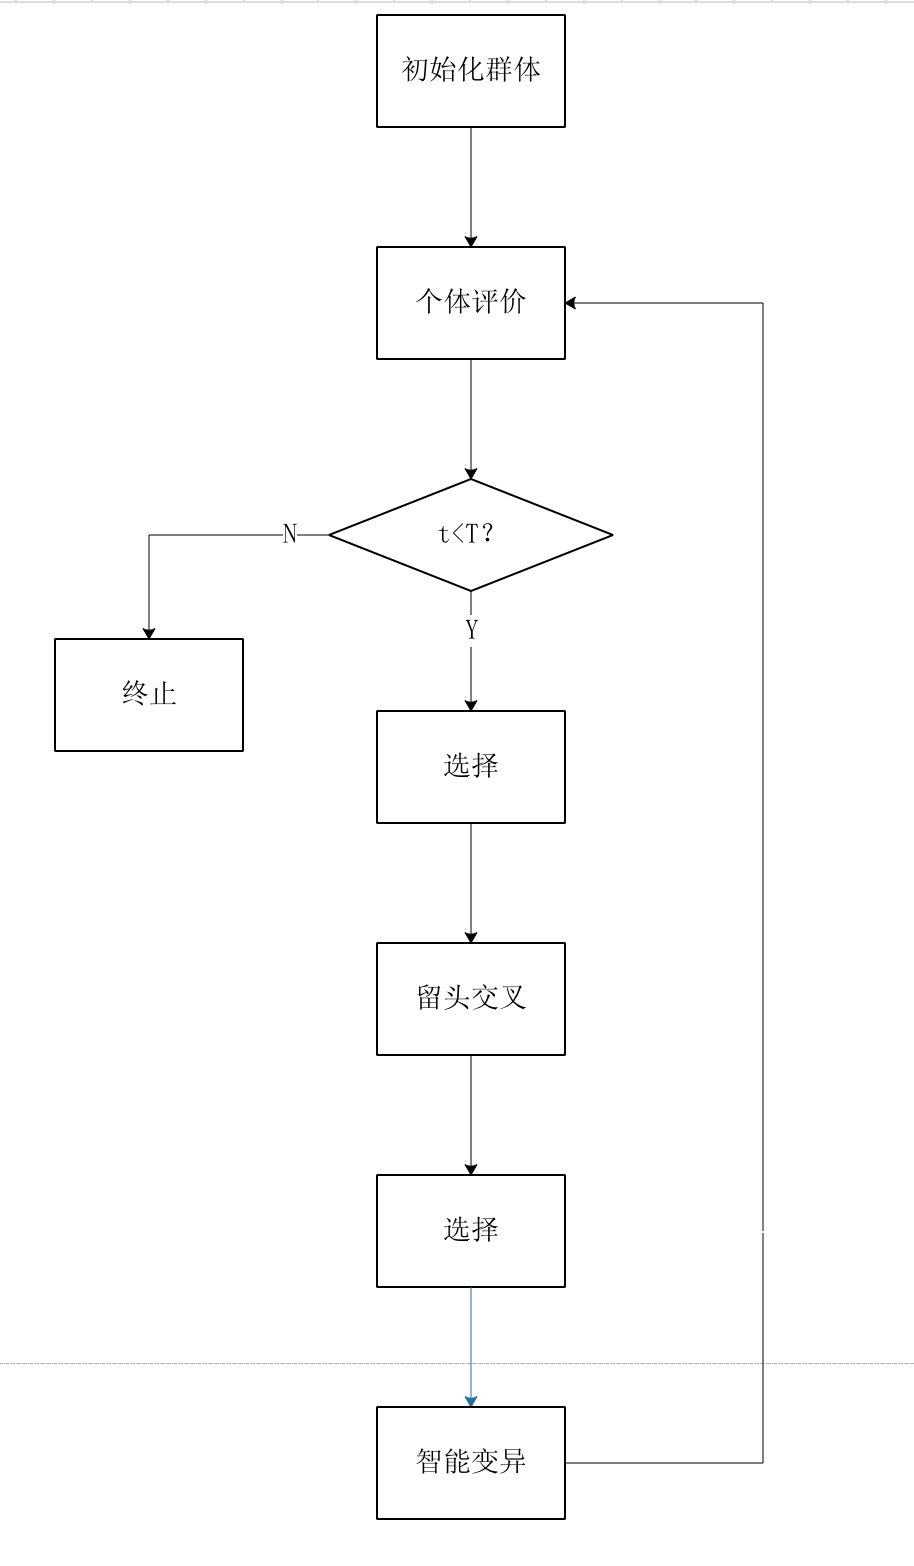
\includegraphics[width=.6\textwidth]{2.png}
\caption{算法流程图}
\end{figure}

我们发现,算法一和算法二得出的结果相同,经过分析,我们得到原因:因为一道工序的加工时间大于为所有CNC上下料、移动、清洗的总时间

由于我们随机生成的数组、父母基因重组产生的新数组,不一定符合RGV调度策略数组的要求。为解决这个问题,我们有两种解决方案。

由于我们目前仅得出两个可行解,而我们对于RGV调度策略数组要求较为严苛,对于一般随机生产出的数组,若它不能通过RGV调度策略数组的编译规则编译,为了初始化群体,为了加快遗传算法的运算效率,我们提出了智能变异的概念
\begin{definition}[智能变异] 
当通过RGV调度策略数组的编译规则编译随机数组失败时,我们对数组的失败节点处的元素进行替换,然后再次编译替换过节点元素的新数组,直至编译成功。
\end{definition}

\begin{definition}[留头交叉] 
在遗传算法进行遗传运算时,父母进行交叉产生后代时,断点前面的基因按照原位传给后代
\end{definition}

对于随机生成的数列,要使其为策略数组的要求:

1、对于随机生产出的数列,若有重复数字位$S_i$的重复数字$S_{i+1}$,则此时,加工时间最久的CNC的加工时间要大于等待时间。

解释:因为在出现重复数字时,由定理1(重复等待定理)可知,此时RGV必为在$S_i$处等待,而等待就意味着其他的CNC还未给RGV发出指令,也即加工时间最久的CNC的加工时间要大于等待时间。

2、对于随机生产出的数列,重复数字不能超过两个。

解释:重复数字如出现三个,在RGV调度策略数组中意味着多次等待,而等待时间没有间隔,多个重复数字占有了多余的基因数目内存,从而这个基因的时间解码结果便会偏低。为加快遗传算法的进化速率和寻优效率,我们对于超过两个的重复数字进行智能变异,以符合我们的需求。

方案一:对于不符合RGV调度策略数组要求的数组,把它直接淘汰


基因重组判断是否能活下来,若不能,遍历不能活下来的数组


同时



根据RGV调度策略数组的特点
再根据我们通过算法一和算法二得出的两组较优解,将这两组解作为


由于我们根据CNC等待时间最短

\bftext{模型求解}
将参数带入附录代码,即可得到最终最优数组、各CNC运行效率、产品生产时间等函数返回值。为验证算法的收敛情况,加入收敛性函数进行检验相邻两代的差异性,公式见下
\begin{equation}
	\sum_{i=1,...,n}^{j=1,...,k}|S^{j+1}_i-S^{j}_i|
\end{equation}
的优化函数的收敛性如下图

问题流程图:












\subsection{一道工序的有故障发生模型}

在一道工序的无故障发生模型中,我们讨论过CNC在不考虑出现故障的情况下的物料加工调度情况。而实际情况中,机器会不可避免地出现损坏、故障等情况。而人工修理机器的过程会占用该机器加工物料时间,这会对于物料加工的调度方案带来一定影响。同时加工时间的缩短,以及正在加工未完成的物料报废也会影响整个智能加工系统的作业效率。因此有必要考虑物料加工作业过程中CNC可能发生故障的情况。

由CNC的作业流程,在情况三下,CNC在某一时刻会处于以下状态三种:

(1)	CNC正在进行正常物料加工;

(2)	CNC已经完成上一物料加工,等待RGV为其上下料;

(3)	CNC在加工过程中出现故障,处于故障状态。

为了简化问题,我们建立状态向量${\bf{C}} = (c(1),c(2),...,c(8))$,其中$c(i)$表示第$i $台CNC的状态 $ (1 \le i \le 8) $,$c(i)$的取值只能为1,0,-1,分别代表上述的状态(1)(2)(3)。这样我们可以清楚地通过状态向量${\bf{C}}$来表示1-8号CNC在某时刻地状态。

假设故障的发生概率约为1\%且故障时间为10-20分钟,即CNC在进行任何一次加工作业,都会有1\%的可能性在加工物料的作业过程中的某一时刻发生10-20分钟的故障。仍考虑一道工序的无故障发生模型中的RGV调度策略数组模拟模型,使用相似的做法,考虑故障:假设故障发生的时刻服从均匀分布,我们在每次CNC上料的同时通过计算机生成一个1-100间的随机小数$r$。如果$r$为小于等于1的小数,则CNC会在该次作业中的某一时刻发生故障,在故障的时刻,该CNC对应的状态向量的元素$c(i)$由1变为-1;如果$r$为大于1的小数,则CNC保持正常的加工状态和后续的等待状态。

若确定某CNC会在一次作业中发生故障,则在CNC作业开始的时刻由计算机生成两个随机数${t_0}$和${t_1}$,分别表示故障时长和故障发生在该次作业的哪个时刻,于是它们的取值范围为${\rm{600}} \le {t_0} \le {\rm{1200}}$,${\rm{0}} \le {t_{\rm{1}}} \le {T_0}$,其中${T_0}$为完成一次加工作业的时间。

分别用向量

\begin{equation}
\begin{array}{l}
{M_1} = ({m_{1}},{m_{12}},{m_{13}},...)\\
{M_2} = ({m_{21}},{m_{22}},{m_{23}},...)\\
{M_3} = ({m_{31}},{m_{32}},{m_{33}},...)
\end{array}
\end{equation}
记录每次故障开始时间,故障结束时间和故障CNC编号。设发生故障的次数为${n}$,则这三个向量的维数:
\begin{equation}
\dim {M_i} = n,i = 1,2,3
\end{equation}
对于第${i}$次故障
,故障开始时间\begin{equation}{m_{1i}} = A({m_{3i}}) + {t_1}\end{equation}
故障结束时间\begin{equation}{m_{2i}} = A({m_{3i}}) + {t_0} + {t_1}\end{equation}
同时$
A(m_{3i})
$
变为
\begin{equation}
A(m_{3i})^{'} = T_0- t_1
\end{equation}
即只有经过${t_1}$秒钟后,该CNC才能回到正常待命状态。







\subsection{两道工序的无故障发生模型}
为了清晰的体现CNC工序安排方案,我们用 \begin{equation}X = (X(1),X(2),...,X(8))\end{equation}标记8台CNC的加工工序,若 $X(i) = 1$,则表示第 台CNC进行第1道工序,否则,进行第2道工序,则所有的CNC工序安排方案共有 $2^8$。我们的目的是在这256种方案中找出一种满足:在该方案下,最优RGV动态调度方案下的产品数目最多。为此,我们建立了目标规划模型。

\subsubsection{产品加工数的求解}
在CNC的每种工序安排方案下,我们均可以寻求相应的最优RGV动态调度方案,并计算这种方案下加工的产品数目。

为了具体反映两道工序无故障情况下的RGV调度特点,我们用 限制RGV下一状态的调度: $ x= 1$,表示接下来RGV可以进行工序1;  $ x= 2$,表示接下来RGV可以进行工序2。则RGV调度策略数组满足:

(1)	若在RGV的第 状态时$ x= 1$,则
\begin{itemize}
\item	当下一个阶段为等待时,$s(i + 1) = s(i)$
\item	当下一个阶段不为等待时,$s(i + 1) \in \{ j|X(j) = 1\} $
\end{itemize}
(2)	若在RGV的第 状态时$ x= 2$,则
\begin{itemize}
\item	当下一个阶段为等待时,$s(i + 1) = s(i)$
\item	当下一个阶段不为等待时,$s(i + 1) \in \{ j|X(j) = 2\} $
\end{itemize}
而判断下一个阶段是否RGV等待、以及不等待时选取合理的CNC进行上下料作业,我们仍旧可以使用一道工序无故障情况下的几种算法,进而求得不同算法下的$n_2^i$。
而对于不同算法,由于考虑角度不一样,并且求得的局部最优解不一定是全局最优解,因此加工的产品数目 可能不一致,我们取
 
\begin{equation}{n_2} = \mathop {\max }\limits_{1 \le i \le 4} \left\{ {n_2^i} \right\}\end{equation}
对应的最优调度方案为s。
\subsubsection{目标规划模型的建立}
由于加工不同工序的CNC的数量以及位置的不同均会导致生产产品数目的不同,我们以8个小时内加工产品数目最多为目标,以每台CNC加工的工序为决策变量,结合$ X(i)$的取值约束:\begin{equation}X(i) = 1,2\end{equation}
\begin{equation}X \ne (1,1,1,1,1,1,1,1)\end{equation}且\begin{equation}X \ne (2,2,2,2,2,2,2,2)\end{equation}即\begin{equation}8 < \sum\limits_{i = 1}^8 {X(i) < 16} \end{equation}
建立目标规划模型,寻求较优的CNC工序安排方案:
 
\begin{equation}\begin{array}{l}
\mathop {\max }\limits_{1 \le j \le 256} \mathop {\max }\limits_{1 \le i \le 4} \left\{ {n_2^{ij}} \right\}\\
s.t.\left\{ \begin{array}{l}
X(i) = 1,2\\
8 < \sum\limits_{i = 1}^8 {X(i) < 16} 
\end{array} \right.
\end{array}\end{equation}
系统作业参数不同那么求得的最优CNC工序安排方案也不同,我们分别将已知的三组数据代入附件的代码,求得不同参数下的最优安排方案以及相应的最优RGV动态调度方案。










\subsection{两道工序的有故障发生模型}








 
\section{模型的评价}
遗传算法的缺点:作为一种随机搜索算法,不能做到全局搜索,因此得到的解不一定是真正的最优解。正如我们所调试的,我们发现遗传算法得出的最优解与我们根据算法1,2得出的结果一致(xxxx)。



%参考文献
\begin{thebibliography}{9}%宽度9
 \bibitem{bib:one} 周永智,吴浩,李怡宁,辛焕海,宋永华. 基于MCS-PSO算法的邻近海岛多微网动态调度[J]. 电力系统自动化,2014,38(09):204-210.
 \bibitem{bib:two} 司守奎,孙玺菁编著.数学建模算法与应用[M].国防工业出版社,201.
\end{thebibliography}

\newpage
%附录
\begin{appendices}
\section{排队算法--matlab 源程序}
\begin{lstlisting}[language=matlab]
kk=2;[mdd,ndd]=size(dd);
while ~isempty(V)
[tmpd,j]=min(W(i,V));tmpj=V(j);
for k=2:ndd
[tmp1,jj]=min(dd(1,k)+W(dd(2,k),V));
tmp2=V(jj);tt(k-1,:)=[tmp1,tmp2,jj];
end
tmp=[tmpd,tmpj,j;tt];[tmp3,tmp4]=min(tmp(:,1));
if tmp3==tmpd, ss(1:2,kk)=[i;tmp(tmp4,2)];
else,tmp5=find(ss(:,tmp4)~=0);tmp6=length(tmp5);
if dd(2,tmp4)==ss(tmp6,tmp4)
ss(1:tmp6+1,kk)=[ss(tmp5,tmp4);tmp(tmp4,2)];
else, ss(1:3,kk)=[i;dd(2,tmp4);tmp(tmp4,2)];
end;end
dd=[dd,[tmp3;tmp(tmp4,2)]];V(tmp(tmp4,3))=[];
[mdd,ndd]=size(dd);kk=kk+1;
end; S=ss; D=dd(1,:);
 \end{lstlisting}
 \section{规划解决程序--lingo源代码}
\begin{lstlisting}[language=c]
kk=2;
[mdd,ndd]=size(dd);
while ~isempty(V)
    [tmpd,j]=min(W(i,V));tmpj=V(j);
for k=2:ndd
    [tmp1,jj]=min(dd(1,k)+W(dd(2,k),V));
    tmp2=V(jj);tt(k-1,:)=[tmp1,tmp2,jj];
end
    tmp=[tmpd,tmpj,j;tt];[tmp3,tmp4]=min(tmp(:,1));
if tmp3==tmpd, ss(1:2,kk)=[i;tmp(tmp4,2)];
else,tmp5=find(ss(:,tmp4)~=0);tmp6=length(tmp5);
if dd(2,tmp4)==ss(tmp6,tmp4)
    ss(1:tmp6+1,kk)=[ss(tmp5,tmp4);tmp(tmp4,2)];
else, ss(1:3,kk)=[i;dd(2,tmp4);tmp(tmp4,2)];
end;
end
    dd=[dd,[tmp3;tmp(tmp4,2)]];V(tmp(tmp4,3))=[];
    [mdd,ndd]=size(dd);
    kk=kk+1;
end;
S=ss;
D=dd(1,:);
 \end{lstlisting}
\end{appendices}

\end{document} 